\documentclass[12pt]{article}

\pagestyle{empty}
\setcounter{secnumdepth}{4}
\setcounter{tocdepth}{4}

\topmargin=0cm
\oddsidemargin=0cm
\textheight=22.0cm
\textwidth=16cm
\parindent=0cm
\parskip=0.15cm
\topskip=0truecm
\raggedbottom
\abovedisplayskip=3mm
\belowdisplayskip=3mm
\abovedisplayshortskip=0mm
\belowdisplayshortskip=2mm
\normalbaselineskip=12pt
\normalbaselines
\usepackage[table]{xcolor}
\usepackage{caption}
\usepackage{graphicx}

\begin{document}

\graphicspath{{C:/Users/Marc/Desktop/ReqDocFolder/}}

\vspace*{0.5in}
\centerline{\bf\Large Requirements Document}

\vspace*{0.5in}
\centerline{\bf\Large Team PI-B}

\vspace*{0.5in}
\centerline{\bf\Large 9 February 2020}

\vspace*{1.0in}
\centerline{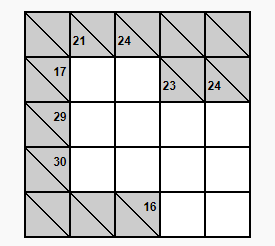
\includegraphics[scale=.75]{KakuroTemp.png}}
\centerline{\bf\Large Kakuro}

\vspace*{0.5in}
\begin{table}[htbp]
\begin{center}
\caption*{Team members}
\begin{tabular}{|c | c|}
\hline
\cellcolor{gray}Name & \cellcolor{gray}ID Number \\
\hline
Sajib Ahmed & A \\
\hline
Yaroslav Bilodid & B \\
\hline
Jesse Desmarais & C \\
\hline
Antoine Farley & D \\
\hline
Marc Hegedus & E \\
\hline
Katerina Tambakis & F \\
\hline
Dmytro Chychkov & G \\
\hline
Yingjie Zhou & H \\
\hline
\end{tabular}
\end{center}
\end{table}

\clearpage

\section{System}

\subsection{Purpose}

\subsection{Context}

\subsection{Business Goals}

\clearpage

\section{Problem Description}
\subsection{Objectives}

The project to be completed in COMP 354 of Winter 2020 is to create a functional replica of the puzzle game Kakuro. Our team's version will comprise of three separate difficulties: easy medium, and hard. The solutions will not be randomly generated, as such it will have three unique working instances. The main objective is to apply software engineering techniques for the developement process to be test-driven, agile, and object-oriented. There will be three iterations, each having their own deadlines. Efficient management and communication amongst our group is understood to be central in accomplishing the required tasks. The client wants the following as deliverables: a basic graphical user interface, a model-view-controller architecture coded in Java, and a categorized set of use cases.\\  
The three iterations will each have a document to be handed in to the client. The information regarding their naming, deliverables, and dates are tabulated below:\\

\begin{table}[htbp]
\begin{center}
\begin{tabular}{| c | c | c |}
\hline
\cellcolor{gray}Iteration & \cellcolor{gray}Deliverable & \cellcolor{gray} Date \\
\hline
Requirement & Requirements Document & 2020/02/09 \\
\hline
Design & Design Document & 2020/03/15 \\
\hline
Implementation & Final Document & 2020/04/5 \\
\hline
\end{tabular}
\caption*{\textit {Project Timeline}}
\end{center}
\end{table}


\subsubsection{Graphical User Interface}
test

\paragraph{Difficulty}\hfill\\ 
\hfill\\
test
\begin{figure}[htbp]
\centerline{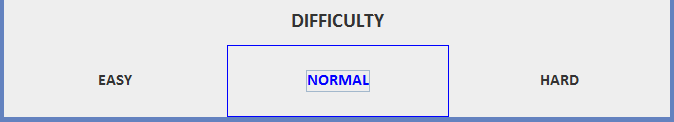
\includegraphics[scale=.75]{difficulty.png}}
\centerline{\textit {Difficulty Interface}}
\end{figure}


\paragraph{GameBoard}\hfill\\ 
\hfill\\
test

\centerline{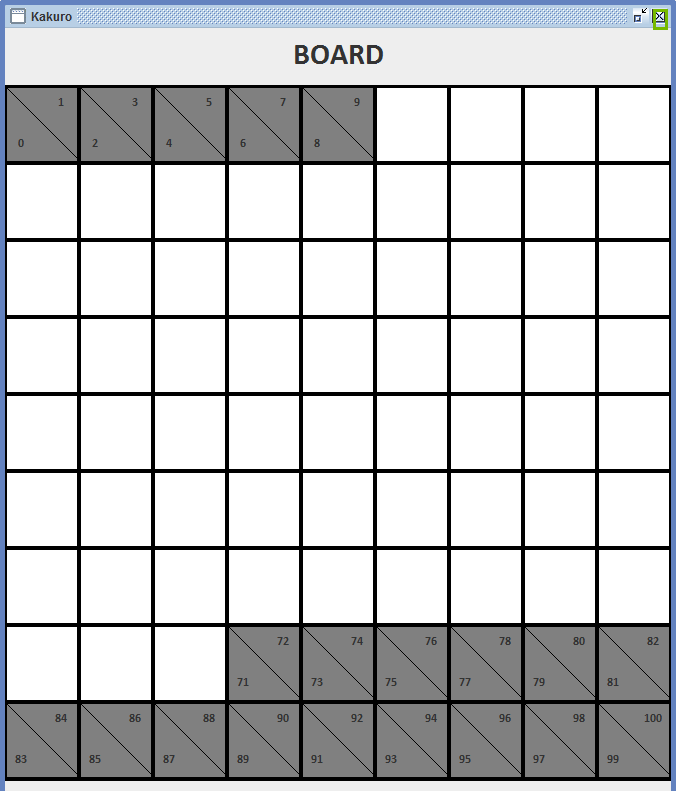
\includegraphics[scale=.75]{gameboard.png}}
\centerline{\textit {Gameboard Display}}

\paragraph{Utilities}\hfill\\ 
\hfill\\
test

\centerline{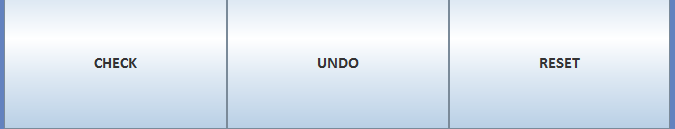
\includegraphics[scale=.75]{utilities.png}}
\centerline{\textit {Utilities Interface}}

\clearpage

\section{Actors}

\clearpage

\section{Use Cases}

\subsection{Overview}

\begin{figure}[htbp]
%insert diagram here
\caption{Use Case Diagram}
\label{fig:use-case-diagram}
\end{figure}

\subsubsection{Use Case 1} \label{uc:1}

\noindent
{\bf Name}\\
Give a name.

\noindent
{\bf Summary}\\
A short summary/description/story.

\noindent
{\bf Actors}\\

\noindent
{\bf Precondition}\\

\noindent
{\bf Main Scenario}\\
\vspace*{-0.2in}
\begin{enumerate}
\item Describe step 1.
\item Describe step 2.
\item Describe step 3.
\end{enumerate}

\noindent
{\bf Exceptions}\\

\noindent
{\bf Postcondition}\\

\noindent
{\bf Priority}\\

\noindent
{\bf Traces to Test Cases}\\
Add when test cases done.

\subsubsection{Use Case 2} \label{uc:2}

\clearpage

\section{Non-Functional Constraints}

\clearpage

\section{Data Dictionary}

\clearpage

\section{References}

\appendix

\section{Description of File Format: Tasks}

Describe input file format.

\section{Description of File Format: Persons}

Describe output file format.

\end{document}
